\documentclass[../Bachelor_Thesis.tex]{subfiles}
 
\begin{document}
Dies ist ein tolles Kapitel!

\begin{figure}[h]
	\begin{subfigure}{0.5\textwidth}
		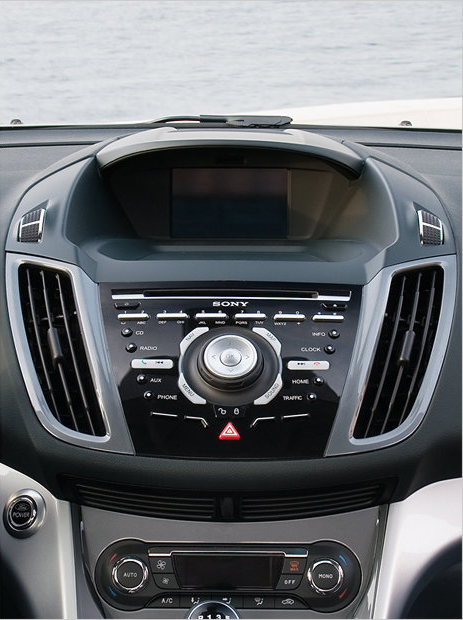
\includegraphics[scale=1.5]{Ford_Radio}
		\caption{Sony Radio and A/C control \cite{Image:Infotainment_Ford_C_Max}}
		\label{fig:Ford_Radio}
	\end{subfigure}
	\begin{subfigure}{0.5\textwidth}
		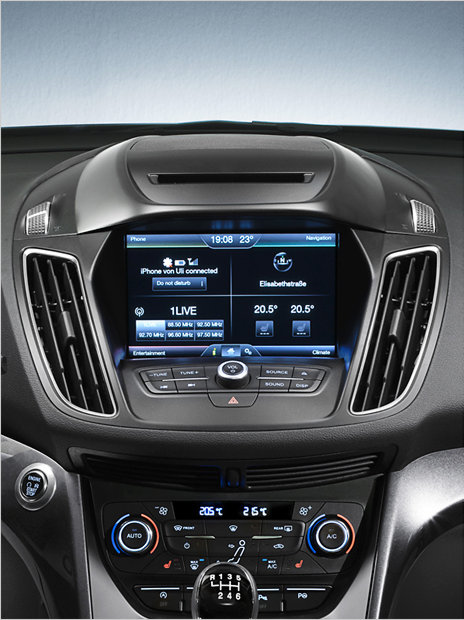
\includegraphics[scale=1.5]{Ford_Infotainmentsystem}
		\caption{Infotainment System \cite{Image:Infotainment_Ford_C_Max}}
		\label{fig:Ford_Infotainmentsystem}
	\end{subfigure}
	\caption{Ford C Max interiors}
\end{figure}


Auf Bild \ref{fig:Ford_Radio} ist ein Autoradio zu sehen.
\cite{Lorensen_Marching_cubes:_A_high_resolut_1987}

\end{document}